% Add common preamble to the document
%% This file is shared between thesis and proposal

\documentclass[a4paper,12pt,twoside]{report}

\usepackage[scaled]{helvet}
\usepackage{url}
\usepackage{cite}
\usepackage{listings}
\usepackage[pdftex]{graphicx}
\usepackage[hang,small,bf]{caption}
\usepackage{styles/tum}
\usepackage{setspace}
\usepackage[german,english]{babel}
\usepackage{float}
\usepackage{floatflt}
\usepackage{fancyhdr}
\usepackage{color}
\usepackage{booktabs}
\usepackage[pdftex,bookmarks=true,plainpages=false,pdfpagelabels=true]{hyperref}	%TODO make yourself familiar with \label, \ref and \hyperref for referencing figures, tables, chapters, etc.
\usepackage{mdwlist}
\usepackage{enumerate}
\usepackage{array}
\usepackage{longtable}
\usepackage[utf8]{inputenc}
\usepackage[capitalize, noabbrev]{cleveref}
\usepackage{wasysym}
\usepackage{todonotes}

% Path for graphics
\graphicspath{{figures/}}

% Include the Thesis metadata like title, author, etc. 
\input{metadata}

%%%%%%%%%%%%%%%%%%%%%%%%%%%%%%%%%%%%%%%%%%%%%%%%%%%%%%%%%%%%%%%%%%%%%%%%%%%%%%%%%%%%%%%%%%%%%%%%%
% Custom Commands for this template
%%%%%%%%%%%%%%%%%%%%%%%%%%%%%%%%%%%%%%%%%%%%%%%%%%%%%%%%%%%%%%%%%%%%%%%%%%%%%%%%%%%%%%%%%%%%%%%%%

% Annotate feedback you received 
\newcommand{\feedback}[1]{\todo[inline,color=green,caption={}]{#1}}

% State what is missing in this spot
\newcommand{\missing}[1]{\todo[inline,color=yellow,caption={}]{#1}}

% Inline to do note: 
\newcommand{\TODO}[1]{\todo[inline,caption={}]{#1}}





\def\proposal{Proposal for}

%%%%%%%%%%%%%%%%%%%%%%%%%%%%%%%%%%%%%%%%%%%%%%%%%%%%%%%%%%%
% Theses specific packages go here
%%%%%%%%%%%%%%%%%%%%%%%%%%%%%%%%%%%%%%%%%%%%%%%%%%%%%%%%%%%
\usepackage[nolist]{acronym}
\usepackage{csquotes}

%%%%%%%%%%%%%%%%%%%%%%%%%%%%%%%%%%%%%%%%%%%%%%%%%%%%%%%%%%%
% Begin of document
%%%%%%%%%%%%%%%%%%%%%%%%%%%%%%%%%%%%%%%%%%%%%%%%%%%%%%%%%%%
\begin{document}
\setlength{\evensidemargin}{22pt}
\setlength{\oddsidemargin}{22pt}


\hypersetup{pdfborder={0 0 0}, pdfauthor={\author}, pdftitle={\title}}

\lstset{showspaces=false, numbers=left, frame=single, basicstyle=\small}

%------- Title setup -------
\thispagestyle{empty}
{
\sffamily

\vspace{1cm}
\begin{center}
\oTUM{4cm}

\vspace{5mm}     
{\LARGE \bf \sffamily Technical University of Munich}

\vspace{5mm}
{\Large School of Computation, Information and Technology \\ -- Informatics -- }	
\vspace{1mm}
\end{center}

\vspace{15mm}

\begin{center}
        {\large {\proposal} {\degree}'s Thesis in \program}
\vspace{8mm}

\begin{spacing}{1.3}
{\LARGE \bf \sffamily \title}\\
\vspace{8mm}

{\LARGE \titleGer}\\
\vspace{8mm}
\end{spacing}

\begin{tabular}{ll}
\large Author:           & \large \author     \\[2mm]
\large Supervisor:       & \large \supervisor \\[2mm]				
\large Advisor:	         & \large \advisor    \\[2mm]
\ifx\proposal\empty\else
\large Start Date:       & \large \startdate  \\[2mm]
\fi
\large Submission Date:  & \large \date
\end{tabular}

\end{center}
}


\selectlanguage{english}
\pagenumbering{arabic}

\fancyhead{}
\pagestyle{fancy}
\fancyhead[LE]{\slshape \leftmark}
\fancyhead[RO]{\slshape \rightmark}
\headheight=15pt

% For wording consistency:
% An "assessment" is a collection of feedbacks + credit scores
% A "feedback" is a single feedback without a score
% A "suggestion" is an assessment that is suggested to a tutor
% A "submission" is a single submission of a student

%------- Start of Proposal -------
\section*{Introduction}
% - Introduce the reader to the general setting
% - What is the environment?
% - What are the tools in use?

% TODO: Briefly explain words from above within the text

The number of students in computer science courses at universities is steadily increasing. At the Technical University of Munich, the number of full-time students\footnote{i.e., full-time equivalents} has recently increased by more than 2,400 within five years~\footnote{TUM in Zahlen 2020, \url{https://mediatum.ub.tum.de/doc/1638190/1638190.pdf}}.
These circumstances present a challenge for instructors, as providing feedback to all students individually can be difficult. Manually graded exercises can provide more individuality, but it is a difficult task to assess all submissions in a timely manner.

Artemis is an online learning platform for exercise management supporting automatic code testing for grading~\cite{ArTEMiS}. The Research Group for Applied Software Engineering at the Technical University of Munich is the main contributor to Artemis, but the system is also in use at several other universities.

Hereafter, we will use the term \textit{submission} to refer to a single submission of a student, \textit{assessment} to refer to a collection of feedbacks and credit scores, and \textit{suggestion} to refer to an assessment that is suggested to a tutor.
Athene, a system for (semi-)automated assessment of text exercises\footnote{\url{https://github.com/ls1intum/Athena}}, is integrated into Artemis~\cite{cofee}. Athene is a microservice-based system written in Python that generates \textit{suggestions} for \textit{assessments} of text exercise \textit{submissions}.


\section*{Problem}
% - What is/are the problem(s)? 
% - Identify the actors and use these to describe how the problem negatively influences them.
% - Do not present solutions or alternatives yet!
% - Present the negative consequences in detail

Currently, Athene is bound to one approach for each step in the assessment generation process. This decreases the flexibility and extensibility of the system and is one of the main points we will improve in this thesis.
On a more practical level, Athene does not support programming exercises, which are a common type of exercise in Computer Science courses. Support for programming exercises is one of the main advantages of Artemis over other exercise management systems (such as Moodle\footnote{\url{https://moodle.org}}), so it would be beneficial to extend Athene to support programming exercises as well.

Two types of actors could have problems with the current status of Athene:
\begin{itemize}
    \item \textbf{Tutors} in courses with manually graded programming exercises: They cannot profit from Athene's assessment generation capabilities, as Athene does not support programming exercises. This means that they won't get any automatically generated suggestions for programming exercises, which would save them a lot of time.
    For textual exercises, Athene currently provides suggestions for around 45\% of the submissions~\cite{cofee2}. In the future, further work might improve this number even further, based on the generalizations of this thesis that allow the system to support different approaches for each step in the assessment generation process.
    \item It is difficult for \textbf{developers} of Athene to integrate additional approaches and features into Athene, as the system is currently bound to one approach for each step in the generation process. Artemis also chooses the assessment suggestions (outside of Athene), which makes it impossible to change the suggestions independently of Artemis.
\end{itemize}

\section*{Motivation}
%- Outline why it is important to solve the problem
% - Again use the actors to present your solution, but don't be to specific
% - Be visionary! 
% - If applicable, motivate with existing research, previous work 

As student numbers will continue to rise (especially in Computer Science courses), the number of assessments which tutors have to make will increase as well. Extending Athene to support programming exercises would allow tutors to profit from its assessment generation capabilities and save them a lot of time.

Others have already recognized the importance of automated assessment generation. For example, the MIT university already developed a system for automated feedback generation on programming assignments in 2013, which corrected 64\% of all submissions on average~\cite{singh2013automated}. However, the system needed access to a reference implementation of the assignment, which is not always available. 
\textit{LetGrade} is another, more recent, automated grading system for prgramming assignments using machine learning techniques, but it does not generate feedback, but only the final grade~\cite{messer2022grading}.

Generalizing each of the steps in the process in Athene would also allow developers to integrate additional approaches and features into Athene more easily.
For example, we could replace the clustering step with a different clustering algorithm, which might improve the quality of the suggestions. Past work like an evaluation of the helpfulness of assessments from Athene~\cite{atheneTracking} or efforts to make it more language-independent~\cite{atheneLanguage} could also potentially have profited from more generalization.

Furthermore, groundwork on a more flexible system might enable applying relatively new innovations like ChatGPT\footnote{\url{https://openai.com/blog/chatgpt}} to Athene, if the suggestion generation does not only support choosing existing assessments, but also generating new ones.

\section*{Objective}
% - What are the main goals of your thesis?
In the thesis, we want to enable Athene to support programming exercises and to generalize the steps in the assessment generation process. We will do this in a way that does not affect the current functionality of Athene and does not introduce any new bugs.

% One of the advantages of having the possibility to choose dynamically between different ways of performing the steps in the assessment generation process is that it would allow us to switch them as necessary to implement suggestions for programming exercises as well. 

\subsection*{Generalization of the Accepted Submission Types}
\begin{figure}[ht]
    \centering
    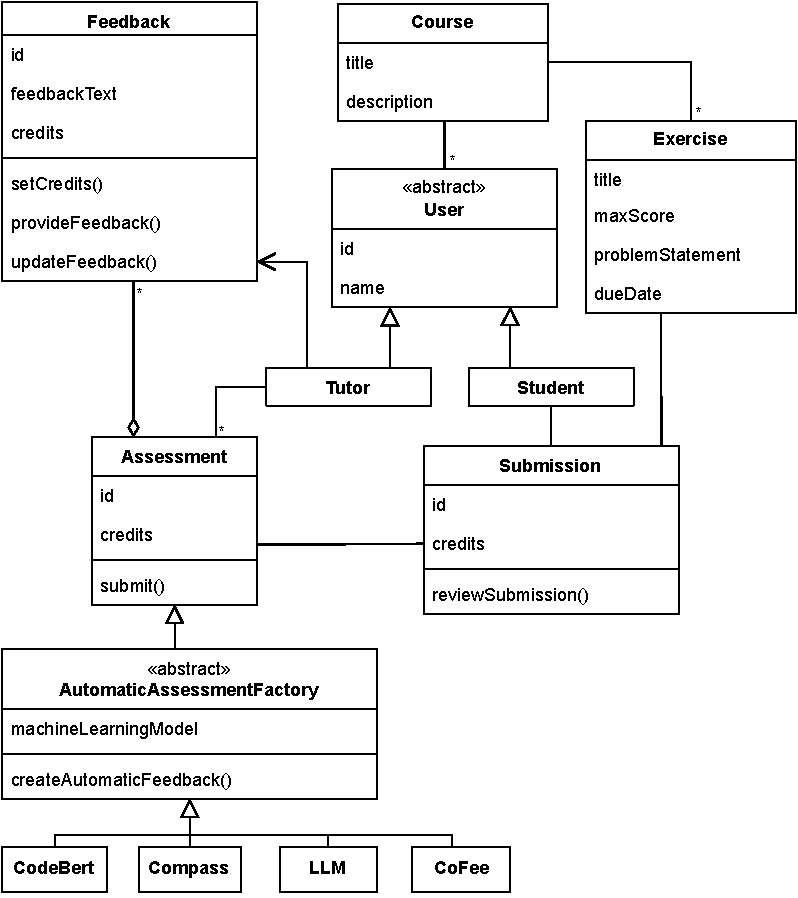
\includegraphics[width=\linewidth]{figures/proposal/aom.pdf}
    \caption{Overview of the current Athene system (AOM diagram), inspired by an AOM diagram created by the CIT team of the iPraktikum, winter semester 2022/23. The \textit{AutomaticFeedbackFactory} will be generalized to support \textit{TextBlock}s from \textit{Submission}s as well as \textit{CodeBlock}s, and potentially more.}
    \label{fig:aom}
\end{figure}
\noindent By moving the actual choice of assessments from Artemis to Athene, we want to make it possible to change the suggestions independently of Artemis. Also, Athene should offer a more general API: Currently, it computes the submission clusters and sends them to Artemis in a ProtoBuf format. A fixed interface contract for the API would make it easier to integrate Athene into other systems in the future. It should be generally possible to process any type of submission with Athene. An overview of the new system is shown in~\cref{fig:aom}.

\subsection*{Generalization of the Processing Steps}
\begin{figure}[ht]
    \centering
    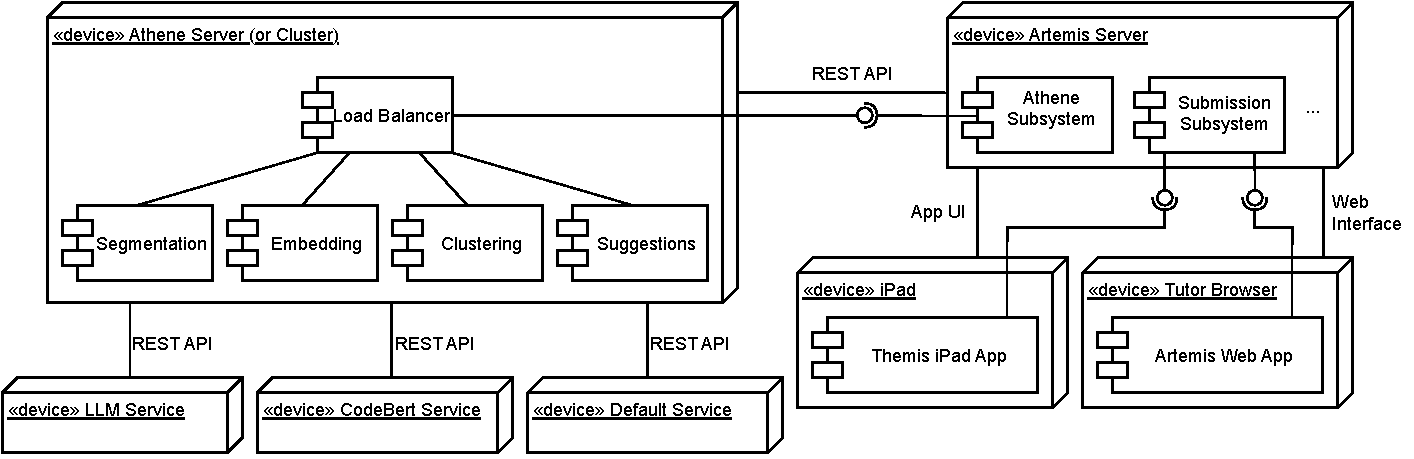
\includegraphics[width=\linewidth]{figures/proposal/deployment.pdf}
    \caption{Overview of the deployment of the targeted system, based on~\cite{atheneLoadBalancer}. The details of the services to perform the calculations are omitted for clarity. Depending on the service, different parts of the system will be activated: For a LLM that directly generates feedback, only the activation of the \textit{Suggestions} component might be necessary. The \textit{Default Service} however, which behaves like the current Athene system, will require the activation of all components.}
    \label{fig:deployment}
\end{figure}
It should be possible to choose between different approaches for determining suggestions. For example, a LLM-based approach could be used for some exercises depending on configuration, while the current approach of clustering submissions could be used for others. The components of the targeted system and their deployment are shown in~\cref{fig:deployment}. The instructor of a course will be able to choose between the different suggestion generation possibilities.

\subsection*{Programming Exercise Assessment Generation}
We will extend Athene to support programming exercises. This will involve extensive analysis of the current state of the art in automatic assessment generation for programming exercises, as well as the development of new approaches for the steps in the generation process. Additionally, we will deploy and test the new system to ensure its reliability and effectiveness.
Existing work on automatic programming exercise assessments~\cite{singh2013automated,messer2022grading} as well as work on automatic source code error detection~\cite{sourceCodeAssessment} might prove useful for this task.

\subsection*{Adding Programming Exercise Suggestions to Artemis}
Because Artemis currently does not support automatic programming exercise suggestions, we also want to make those available in Artemis. Tutors should be able to accept or reject the suggestions in the web interface, similar to the existing automatic assessments on text exercises, which Athene generates. 

\subsection*{Adding Programming Exercise Suggestions to Themis}

Themis\footnote{\url{https://github.com/ls1intum/Themis}} is a new iPad app, which supports grading of programming exercises. The app was a project in the practical course \enquote{iPraktikum} at the Technical University of Munich.
Themis will also be able to use the programming exercise suggestions from Athene. It should do so by only communicating with Artemis directly, which means that Themis will not need to communicate with Athene directly. This decreases the coupling between Themis and Athene and makes it easier to change the generation system in the future.

\subsection*{Iterating on Existing Work from ThemisML}
Currently, Themis supports automatic suggestions for programming exercises by using its own assessment generation system prototype, ThemisML\footnote{\url{https://github.com/ls1intum/Themis-ML}}.
Parts of this system will be useful for integrating programming exercise suggestions into Athene. ThemisML uses codeBERT~\cite{codeBERT} to compute pairwise similarity scores between submissions to suggest appropriate suggestions. We want to move this functionality into Athene to completely replace the current generation system in ThemisML.

\subsection*{Utilizing codeBERT for Assessment Generation}
We will evaluate a variety of approaches for effectively segmenting, embedding and clustering programming exercises to improve on the efficiency and quality of the suggestions and to integrate them into Athene.
One of the main approaches we will evaluate is codeBERT~\cite{codeBERT}, which is a BERT model that was trained on code. Currently it is used in ThemisML to compute pairwise similarity scores between submissions. We will evaluate how it can be used in a more general assessment generation system.


\section*{Schedule}
% - When will the thesis Start (Always 15th of Month) 
% - Create a rough plan for your thesis (separate the time in sprints with a length of 2-4 Weeks)
% - Each sprint should contain several work items - Again keep it high-level and make to keep your plan realistic
% - Make sure the work-items are measurable and deliverable 
% - No writing related tasks! (e.g. "Write Analysis Chapter")

The following schedule roughly outlines the work items for the thesis. It will start on March 15th, 2023 and last for 6 months, roughly 26 weeks.

\begin{itemize}
    \item \textbf{Sprint 1 (Week 1--2)}: Requirements Gathering \& Preparation
    \begin{itemize}
        \item Create a requirements document for the new system.
        \item Familiarize with the existing code base of Athene and Artemis, especially the assessment choice within Artemis.
        \item Evaluate different approaches for automatic assessment generation for programming exercises.
    \end{itemize}
    \item \textbf{Sprint 2 (Week 3--5)}: System Design Generalization
    \begin{itemize}
        \item Analyze the current architecture of Athene and evaluate alternatives.
        \item Design an architecture for easily switching the code executed in each step by Athene.
        \item Refactor the existing microservices to use the new architecture.
        \item Verify that the new architecture works as before.
    \end{itemize}
    \item \textbf{Sprint 3 (Week 6--7)}: Suggestion Generation Analysis
    \begin{itemize}
        \item Thoroughly analyze the current implementation of the suggestion generation in Artemis.
        \item Develop a small locally running prototype in Python that roughly resembles the current Java implementation.
    \end{itemize}
    \item \textbf{Sprint 4 (Week 7--9)}: Suggestion Creation Endpoint
    \begin{itemize}
        \item Improve on the prototype from Sprint 3.
        \item Design a new API endpoint for Athene that can be used to generate suggestions for programming exercises, with emphasis on modularity and extensibility.
        \item Implement a new microservice in Athene for this endpoint.
        \item Test the new microservice.
    \end{itemize}
    \item \textbf{Sprint 5 (Week 10--11)}: Suggestion Generation Refactoring in Artemis
    \begin{itemize}
        \item Refactor the current suggestion generation in Artemis to use the new endpoint, while keeping the current functionality.
        \item Manually and automatically test the changes in Artemis.
        \item Identify potential improvements for the new system.
    \end{itemize}
    %! 11-12
    \item \textbf{Sprint 6 (Week 12--13)}: Suggestion Generation Improvements
    \begin{itemize}
        \item Identify issues and improvements to the new system. Implement them.
        \item Add a new control in Artemis to switch between different suggestion generation systems.
        \item Test the new system.
    \end{itemize}
    \item \textbf{Sprint 7 (Week 14--15)}: Evaluation of Automatic Processing of Programming Exercises
    \begin{itemize}
        \item Evaluate codeBERT as a possible approach for automatic assessment generation for programming exercises.
        \item Evaluate other approaches for automatic assessment generation for programming exercises, also using the findings from Sprint 1.
        \item Find the best way of segmenting the submissions, e.g. based on method blocks (like in ThemisML) or based on other metrics.
    \end{itemize}
    \item \textbf{Sprint 8 (Week 16--19)}: Support for Programming Exercises
    \begin{itemize}
        \item Add support for programming exercise segmentation, embedding and clustering as well as suggestion generation to Athene - based on prior research.
        \item Gather data for the evaluation of the new system.
        \item Evaluate the new system and compare it to ThemisML.
    \end{itemize}
    \item \textbf{Sprint 9 (Week 20--22)}: Displaying Suggestions in Artemis and Themis
    \begin{itemize}
        \item Add support for displaying automatic suggestions for programming exercises in Artemis.
        \item Add support for displaying automatic suggestions for programming exercises in Themis.
        \item Test the new systems.
    \end{itemize}
    \item \textbf{Sprint 10 (Week 23--26)}: Final Improvements, Documentation on How to Create New Assessment Generators and an Assessment Generator Template
    \begin{itemize}
        \item Improve on issues from previous sprints.
        \item Create documentation on how to create new assessment generators. This should show how to connect to the interfaces provided by the new system within Athene, how to create a new assessment generator and how to test it.
        \item Create a template for new assessment generators in Python.
    \end{itemize}

\end{itemize}


\clearpage
\begin{acronym}
\acro{GUI}{Graphical User Interface}
\end{acronym}

\clearpage
\bibliography{thesis}
\bibliographystyle{alpha}

\end{document}
